\song{Holubí dům (Jiří Schelinger)}
\begin{multicols}{2}
\re{}(capo 1)

\ve{}
\ch{Am G}Zpívám \ch{F}ptákům a \ch{E}zvlášť holu\ch{Am}bům,\\
\ch{Am G}stával v \ch{F}{ú}dolí \ch{E}mém starý \ch{Am}dům.\\
\ch{C}Ptá\ch{G}ků \ch{C}houf \ch{G}zalétal ke kro\ch{C}vům,\\
\ch{Am}měl \ch{G}jsem \ch{F}rád holu\ch{E}bích křídel \ch{Am}{š}um.

\ve{}
Vlídná dívka jim házela hrách,\\
mávání perutí víří prach.\\
Ptáci krouží a neznají strach,\\
měl jsem rád starý dům, jeho práh.

\cho{}
Hledám \ch{Dm}dům holu\ch{G}bí,\\
kdopak z \ch{C}vás cestu \ch{Am}ví,\\
míval \ch{Dm}stáj roube\ch{G}nou, bílý \ch{C}{š}tít.\\
Kde je \ch{F}dům holu\ch{G}bí a ta \ch{C}dívka kde \ch{Am}spí,\\
vždyť to \ch{Dm}ví, že jsem \ch{E}chtěl pro ni \ch{Am}{ž}ít.

\ve{}
Sdílný déšť vypráví okapům,\\
bláhový, kdo hledá tenhle dům.\\
Odrůstáš chlapeckým střevícům,\\
neslyšíš holubích křídel šum.

\ve{}
Nabízej úplatou cokoli,\\
nepojíš cukrových homolí.\\
Můžeš mít třeba zrak sokolí,\\
nespatříš ztracené údolí.

\re{*}
\ch{Am G}Zpvám \ch{F}ptákům a \ch{E}zvlášť holu\ch{Am}bům,\\
stával v údolí mém starý dům.

\columnbreak
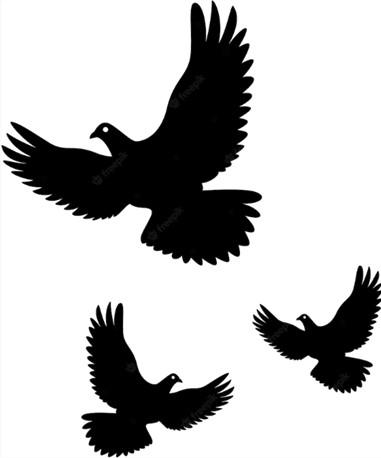
\includegraphics[width = \columnwidth]{images/holubi_dum.jpg}
\end{multicols}
\esong{}